\documentclass[english, aspectratio=169]{beamer}
% english is for the language used in standard texts (figures, tables etc)
% aspectratio of 16:9 or set it for more old school to 4:3 (without the ':')

% ---------------------------------------------------------------------------- %
% Load base preamble
% ---------------------------------------------------------------------------- %
\usepackage{import}
\subimport{../preamble/}{beamer.tex}

% ---------------------------------------------------------------------------- %
% Local settings
% ---------------------------------------------------------------------------- %
% https://tex.stackexchange.com/a/20613
\newcommand\hcancel[2][black]{\setbox0=\hbox{$#2$}%
  \rlap{\raisebox{.35\ht0}{\textcolor{#1}{\rule{\wd0}{1pt}}}}#2}

\newcommand{\B}[0]{\ensuremath{\mathbb{B}}}
\newcommand{\pow}[0]{\ensuremath{\mathcal{P}}}

\newcommand{\sort}[0]{\text{sort}}

\newcommand{\triple}[3]{\ensuremath{(#1, #2, #3)}}
\renewcommand{\arc}[3]{\ensuremath{#1 \xrightarrow{_{#2}} #3}}

\tikzstyle{plot_adiar}=[color=blue, mark=o, mark size=1.5pt, line width=1pt]
\tikzstyle{plot_cudd}=[color=red, mark=diamond, mark size=1.5pt, line width=1pt]

% Horizontal legends: https://tex.stackexchange.com/a/101578
% argument #1: any options
\makeatletter
\newenvironment{customlegend}[1][]{%
    \begingroup
    % inits/clears the lists (which might be populated from previous
    % axes):
    \pgfplots@init@cleared@structures
    \pgfplotsset{#1}%
}{%
    % draws the legend:
    \pgfplots@createlegend
    \endgroup
}%

% makes \addlegendimage available (typically only available within an
% axis environment):
\def\addlegendimage{\pgfplots@addlegendimage}
\makeatother

% ------------------------------------------------------------------------------
% TITLEPAGE
% ------------------------------------------------------------------------------
\title{
  Adiar 1.1 : Zero-suppressed Decision Diagrams\\\hspace{80pt}in External Memory
}

\author{{\bf Steffan Christ S{\o}lvsten} and Jaco van de Pol}

\institute{
\includegraphics[width=0.2\linewidth]{../external/aulogo_uk_var2_black.eps}}

\date{$18^{\text{th}}$ of May, 2023}

\begin{document}

\titleframe

\begin{frame}[b,plain,noframenumbering]{}
  \pause

  \begin{center}
    {\Huge \textbf{Adiar}}

    {\large
      \only<-2>{%
        Binary%
      }%
      \only<3>{%
        {\textbf{Multi-terminal}}%
      }%
      \only<4>{%
        {\textbf{Quantum Multi-valued}}%
      }%
      \only<5>{%
        {\textbf{Zero-suppressed}}%
      }
      Decision Diagrams

      \vspace{-5pt}
      in External Memory
    }

    \vspace{12pt}

    \textcolor{gray}{\small
      \href{http://github.com/ssoelvsten/adiar}{github.com/ssoelvsten/adiar}
    }

    \vspace{80pt}
  \end{center}
\end{frame}

\begin{frame}
  \begin{figure}
    \centering

    \begin{tikzpicture}[every node/.style={transform shape}]
      % nodes
      \node[shape = circle, draw = black]
      (0) {$x_0$};

      \node[shape = circle, draw = black, below left=1.4cm and .5cm of 0]
      (21) {$x_2$};

      \node[shape = circle, draw = black, below right=1.4cm and .5cm of 0]
      (22) {$x_2$};

      \node[shape = circle, draw = black, below right=0.4cm and .5cm of 21]
      (3) {$x_3$};

      % leafs
      \node[shape = rectangle, draw = black, below left=.4cm and .5cm of 3]
      (sink_F) {$0$};

      \node[shape = rectangle, draw = black, below right=.4cm and .5cm of 3]
      (sink_T) {$1$};

      % arcs
      \draw[->, dashed]
      (0)  edge (21)
      (21) edge (sink_F)
      (22) edge (3)
      (3)  edge (sink_F)
      ;

      \draw[->]
        (0)  edge (22)
        (21) edge (3)
        (22) edge (sink_T)
        (3)  edge (sink_T)
      ;

      % semantics
      \onslide<2>{
        \node[below right=0.1cm and 0.4cm of 0] {$x_0 = 1$};
        \node[below left=0.1cm and 0.4cm of 0]  {$x_0 = 0$};
      }
    \end{tikzpicture}
  \end{figure}
\end{frame}

\begin{frame}
  \begin{figure}
    \centering

    \begin{subfigure}[b]{0.32\linewidth}
      \centering

      \begin{tikzpicture}[every node/.style={transform shape}]
        \node[shape = circle, black, draw = black] (i) {$x_i$};
\node[shape = circle, draw = black, below=of i] (child) {};
\node[shape = circle, draw = black, above=of i] (parent) {};

% implication
\node[shape = circle, black,right=0.5cm of i] {$\implies$};

% after
\node[shape = circle, draw = black, right=2.5cm of child] (childafter) {};
\node[shape = circle, draw = black, right=2.5cm of parent] (parentafter) {};

\draw[->, dashed] (i) edge[bend right] (child);
\draw[->]
(i) edge[bend left] (child)
(parent) edge (i)
(parentafter) edge (childafter)
;

      \end{tikzpicture}

      \vspace{10pt}
      {\small {\bf BDD: } $f : \B^n \rightarrow \B$}
    \end{subfigure}
    \qquad\pause
    \begin{subfigure}[b]{0.32\linewidth}
      \centering

      \begin{tikzpicture}[every node/.style={transform shape}]
        \node[shape = circle, black, draw = black] (i) {$x_i$};
\node[shape = circle, draw = black, below left=1.2 and 0 of i] (child) {};
\node[shape = rectangle, draw = black, below right=1 and 0 of i] (terminal) {$0$};

\node[shape = circle, draw = black, above=of i] (parent) {};

% implication
\node[shape = circle, black,right=0.5cm of i] {$\implies$};

% after
\node[shape = circle, draw = black, right=2.4cm of child] (childafter) {};
\node[shape = circle, draw = black, right=2cm of parent] (parentafter) {};

\draw[->, dashed] (i) edge[bend right=5] (child);
\draw[->]
  (i) edge[bend left=5] (terminal)
  (parent) edge (i)
  (parentafter) edge (childafter)
;

      \end{tikzpicture}

      \vspace{10pt}
      {\small {\bf ZDD: } $A \subseteq \pow(\B^n)$}
    \end{subfigure}
  \end{figure}
\end{frame}

\begin{frame}
  \begin{figure}
    \centering

    \begin{tikzpicture}
      \node[shape=circle, draw=black] at (1,0) (prod2) {};
      \node[above=0.4 of prod2] (bdd_apply) {\texttt{bdd\_apply}};
      \node[below=0.4 of prod2] (zdd_binop) {\texttt{zdd\_binop}};

      \draw[->, rounded corners, line width = 1.2pt]
        (prod2) edge (zdd_binop)
        (prod2) edge (bdd_apply)
      ;

      \onslide<2-> {
        \node[shape=circle, draw=black] at (5,0) (substitute) {};
        \node[below=0.4 of substitute] (zdd_onset)    {\texttt{zdd\_onset}};
        \node[right=0.4 of substitute] (bdd_restrict) {\texttt{bdd\_restrict}};
        \node[above=0.4 of substitute] (zdd_offset)   {\texttt{zdd\_offset}};

        \draw[->, rounded corners, line width = 1.2pt]
          (substitute) edge (zdd_onset)
          (substitute) edge (bdd_restrict)
          (substitute) edge (zdd_offset)
        ;
      }

      \onslide<2-> {
        \node[shape=circle, draw=black] at (-3,0) (count) {};
        \node[above=0.4 of count] (bdd_pathcount) {\texttt{bdd\_pathcount}};
        \node[below=0.4 of count] (zdd_size)      {\texttt{zdd\_size}};

        \draw[->, rounded corners, line width = 1.2pt]
          (count) edge (bdd_pathcount)
          (count) edge (zdd_size)
        ;
      }

      \onslide<2-> {
        \node[shape=circle, draw=black] at (-1.8,-3) (pred) {};
        \node[left=0.4  of pred] (zdd_equal)    {\texttt{zdd\_equal}};
        \node[below=0.4 of pred] (zdd_subseteq) {\texttt{zdd\_subseteq}};
        \node[right=0.4 of pred] (bdd_equal)    {\texttt{bdd\_equal}};
        \node[above=0.4 of pred] (zdd_disjoint) {\texttt{zdd\_disjoint}};

        \draw[->, rounded corners, line width = 1.2pt]
          (pred) edge (zdd_equal)
          (pred) edge (zdd_subseteq)
          (pred) edge (bdd_equal)
          (pred) edge (zdd_disjoint)
        ;
      }

      \onslide<4> {
        \node[shape=circle, draw=black] at (4.8,-3) (intercut) {};
      }
      \onslide<3-> {
        \node[left=0.4  of intercut] (zdd_change)             {\texttt{zdd\_change}};
        \node[below=0.4 of intercut] (zdd_complement)         {\texttt{zdd\_complement}};
        \node[right=0.4 of intercut] (zdd_expand)             {\texttt{zdd\_expand}};
        \node[above right=0.4 and 0.6 of intercut] (zdd_from) {\texttt{zdd\_from\_bdd}};
        \node[above left =0.4 and 0.6 of intercut] (bdd_from) {\texttt{bdd\_from\_zdd}};
      }

      \onslide<4> {
        \draw[->, rounded corners, line width = 1.2pt]
          (intercut) edge (zdd_change)
          (intercut) edge (zdd_complement)
          (intercut) edge (zdd_expand)
        ;
        \draw[->, rounded corners, line width = 1.2pt]
          (intercut) |- (zdd_from)
        ;
        \draw[->, rounded corners, line width = 1.2pt]
          (intercut) |- (bdd_from)
        ;
      }
    \end{tikzpicture}

  \end{figure}
\end{frame}

\begin{frame}[plain,noframenumbering]{}
  \Large

  \only<1->{\texttt{zdd\_binop($A$, $B$, $\otimes$) =}}
  \only<1>{\texttt{prod2($A$, $B$, $\otimes$, zdd\_strategy)}}%
  \only<2>{\texttt{prod2<zdd\_policy>($A$, $B$, $\otimes$)}}
\end{frame}

\begin{frame}
  \begin{figure}
    \centering

    \setvalue{arch_adiar = gray}
    \setvalue{arch_internal = gray}
    \setvalue{arch_bdd = gray}
    \setvalue{arch_zdd = gray}

    \only<1> {
      \setvalue{arch_bdd = white}
      \setvalue{arch_zdd = white}
      \setvalue{arch_internal = black}
    }

    \only<2> {
      \setvalue{arch_bdd = black}
      \setvalue{arch_zdd = black}
    }

    \only<3> {
      \setvalue{arch_internal = black}
    }

    \begin{tikzpicture}
      % <adiar>
\draw[densely dotted, color=black] (0,0) rectangle ++(11.5,6);
\node[anchor=west, color=black] at (0,5.8) {\footnotesize \emph{\texttt{<adiar>}}};

\node[color=black] at (5.7,5.5) {$\dots$};

% <adiar/internal>
\draw[densely dotted, color=\getvalue{arch_internal}] (0.2,0.2) rectangle ++(11.1,1.7);
\node[anchor=west, color=\getvalue{arch_internal}] at (0.2,1.7) {\footnotesize \emph{\texttt{<adiar/internal>}}};

\node[draw, rectangle split, rectangle split parts=2, color=\getvalue{arch_internal}]
at (5.7, 1) (internal_prod2)
{ \footnotesize \texttt{prod2.h} \nodepart{two}
  \footnotesize \texttt{prod2<$\dots$>($\dots$)}
};

\node[color=\getvalue{arch_internal}] at (8,1) {$\dots$};

% <adiar/bdd>
\draw[densely dotted, color=\getvalue{arch_bdd}] (0.2,2.4) rectangle ++(5.2,2.5);
\node[anchor=west, color=\getvalue{arch_bdd}] at (0.2,4.7) {\footnotesize \emph{\texttt{<adiar/bdd>}}};

\node[draw, rectangle split, rectangle split parts=2, color=\getvalue{arch_bdd}]
at (3.4,3.5) (bdd_apply)
{ \footnotesize \texttt{bdd\_apply.cpp} \nodepart{two}
  \footnotesize
  \begin{tabular}{l}
    \texttt{bdd\_prod2\_policy}
    \\
    \texttt{bdd\_apply($\dots$)}
  \end{tabular}
};

\node[color=\getvalue{arch_bdd}] at (0.9,3.5) {$\dots$};

\draw[->, rounded corners, line width = 0.7pt, dashed, color=\getvalue{arch_bdd}]
  (internal_prod2) -- ($(internal_prod2)+(0,1.1)$) -| (bdd_apply);

% <adiar/zdd>
\draw[densely dotted, color=\getvalue{arch_zdd}] (6,2.4) rectangle ++(5.2,2.5);
\node[anchor=west, color=\getvalue{arch_zdd}] at (6,4.7) {\footnotesize \emph{\texttt{<adiar/zdd>}}};

\node[draw, rectangle split, rectangle split parts=2, color=\getvalue{arch_zdd}]
at (8,3.5) (zdd_binop)
{ \footnotesize \texttt{zdd\_binop.cpp} \nodepart{two}
  \footnotesize
  \begin{tabular}{l}
    \texttt{zdd\_prod2\_policy}
    \\
    \texttt{zdd\_binop($\dots$)}
  \end{tabular}
};

\node[color=\getvalue{arch_zdd}] at (10.5,3.5) {$\dots$};

\draw[->, rounded corners, line width = 0.7pt, dashed, color=\getvalue{arch_zdd}]
  (internal_prod2) -- ($(internal_prod2)+(0,1.1)$) -| (zdd_binop);

    \end{tikzpicture}
  \end{figure}
\end{frame}

\blankframe

\begin{frame}
  \begin{figure}
    \centering

    \begin{tikzpicture}
      \begin{axis}[%
        width=0.80\linewidth, height=0.42\linewidth,
        every tick label/.append style={font=\scriptsize},
        % x-axis
        xlabel={Number of ZDD nodes},
        xmajorgrids=true,
        xmin=10000000,
        xmax=1000000000000,
        xmode = log,
        % y-axis
        ymin=0,
        ymax=4,
        ytick distance={0.5},
        ylabel={$\mu$s / ZDD node},
        yminorgrids=true,
        ymajorgrids=true,
        grid style={dashed,black!20},
        ]

        \only<2-> {
          \addplot+ [style=plot_cudd]
          table {./data/tic_tac_toe_zdd_cudd_time_per_node.tex};
        }
        \only<2-> {
          \addplot+ [style=plot_adiar]
          table {./data/tic_tac_toe_zdd_adiar_v1-1-0_time_per_node.tex};
        }
      \end{axis}
      \only<2-> {
        \node[color=black] at (6.5, 1.35) {\footnotesize $16.9$~GiB};
      }
      \only<3-> {
        \node[color=black] at (8.4, 1.9)  {\footnotesize $130.8$~GiB};
        \node[color=black] at (8.8, 3.95) {\footnotesize $838.9$~GiB};
      }
    \end{tikzpicture}

    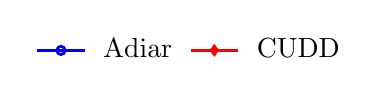
\begin{tikzpicture}
      \begin{customlegend}[
        legend columns=-1,
        legend style={draw=none,column sep=1ex},
        legend entries={Adiar, CUDD}
        ]
        \addlegendimage{style=plot_adiar}
        \addlegendimage{style=plot_cudd}
      \end{customlegend}
    \end{tikzpicture}

    \caption{Running time for \emph{Tic-Tac-Toe} with $300$~GiB of RAM.}
  \end{figure}
\end{frame}

\blankframe

\begin{frame}
  \begin{figure}
    \centering

    \begin{tikzpicture}
      % Done(ish) [2]
      \node at (0,-2) (bdd) {BDD};
      \node[right=1 of bdd] (zdd) {ZDD};

      \onslide<2-> {
        \node[left=1 of bdd] (fdd) {FDD};
      }

      \onslide<3-> {
        \node[shape=rectangle, draw=black] at (0,0)
          (ptr_t) {\texttt{ptr\_t}};

        % Multi-terminal BDD
        \node[right=3 of ptr_t] (mtbdd) {MTBDD};
        \draw[->, rounded corners, line width = 1.2pt]
          (ptr_t) edge node[above] {\em + terminal type} (mtbdd);
      }

      \onslide<4-> {
        % Tagged BDD
        \node[below left=0.5 and 1.4 of ptr_t] (tbdd) {TBDD};
        \draw[->, rounded corners, line width = 1.2pt]
          (ptr_t) -- node[above left=-0.1 and 0] {\em + weight}  ($(ptr_t)+(-1,0)$) -| (tbdd);
        }

      \onslide<5-> {
        \node[below left=-0.56 and -0.3 of fdd] (kfdd) {(K)};

        \draw[->, rounded corners, line width = 1.2pt]
          (tbdd) -- (kfdd);
      }

      \onslide<6-> {
        \node[shape=rectangle, draw=black] at (0,2.5)
          (node_t) {\texttt{node\_t}};

        % LDD and Chained BDD
        \node[above right=0.3 and 0.8 of node_t] (ldd) {\qquad\quad LDD (MDD)};
        \node[below right=0.3 and 1.2 of node_t] (chained) {Chained BDDs};

        \draw[->, rounded corners, line width = 1.2pt]
          (node_t) -- node[above right=-0.1 and 0] {\em + weight}  ($(node_t)+(1,0)$) -| (ldd);
        \draw[->, rounded corners, line width = 1.2pt]
          (node_t) -- ($(node_t)+(1,0)$) -| (chained);
      }

      \onslide<7-> {
        % QMDD
        \node[below left=0.75 and 1.9 of node_t] (qmdd) {QMDD};

        \draw[->, rounded corners, line width = 1.2pt]
          (node_t) -- node[above left=-0.1 and 0] {\em + out-degree}  ($(node_t)+(-1,0)$) -| (qmdd);
        \draw[->, rounded corners, line width = 1.2pt]
          (ptr_t) -- ($(ptr_t)+(-1,0)$) -| (qmdd);
      }
    \end{tikzpicture}
  \end{figure}
\end{frame}

\begin{frame}[plain,noframenumbering]
  {\Large \textbf{Steffan Christ Sølvsten}}
  \vspace{1pt} {\hrule width0.45\linewidth}

  \vspace{5pt}

  \begin{itemize}
  \item[\faIcon{envelope}] \mailto{soelvsten@cs.au.dk}
  \item[\faIcon{twitter}] \href{https://www.twitter.com/ssoelvsten}{@ssoelvsten}
  \end{itemize}

  \vspace{10pt}

  {\Large \textbf{Adiar}}
  \vspace{1pt} {\hrule width0.45\linewidth}

  \vspace{5pt}

  \begin{itemize}
  \item[\faIcon{code}]
    \href{http://github.com/ssoelvsten/adiar}{github.com/ssoelvsten/adiar}
  \item[\faIcon{book}\hspace{2pt}]
    \href{http://ssoelvsten.github.io/adiar}{ssoelvsten.github.io/adiar}
  \end{itemize}


  \vspace{10pt}

  
\includegraphics[width=0.2\linewidth]{external/aulogo_uk_var2_black.eps}
\end{frame}

\begin{frame}
  \begin{columns}
  \begin{column}{0.49\textwidth}

    \begin{figure}
      \centering

      \begin{subfigure}{1\linewidth}
        \centering

        \begin{tikzpicture}[scale=0.9, every node/.style={transform shape}]
          % nodes
          \node[shape = circle, draw = black]
          (0) {\tiny $(0,0)$};

          \node[shape = circle, draw = black, below right= .3cm and .5cm of 0]
          (1) {\tiny $(1,0)$};

          \node[shape = circle, draw = black, below left=.3cm and .5cm of 1]
          (2) {\tiny $(2,0)$};

          \node[shape = circle, draw = black, below left=.3cm and .5cm of 2]
          (31) {\tiny $(3,0)$};
          \node[shape = circle, draw = black, below right=.3cm and .5cm of 2]
          (32) {\tiny $(3,1)$};

          % leafs
          \node[shape = rectangle, draw = black, below=.4cm of 31]
          (sink_T) {$\top$};

          \node[shape = rectangle, draw = black, below=.4cm of 32]
          (sink_F) {$\bot$};

          % arcs
          \draw[->,dashed]
          (0) edge (2)
          (1) edge (2)
          (2) edge (31)
          (31) edge (sink_T)
          (32) edge (sink_F)
          ;

          \draw[->]
          (0) edge (1)
          (1) edge (32)
          (2) edge (32)
          (31) edge (sink_F)
          (32) edge (sink_T)
          ;

          % animations
          \onslide<3-5>{ % 0
            \node[shape = circle, orange, draw = orange]
            {\tiny $(0,0)$};
            \draw[->,dashed,orange] (0) edge (2);
            \draw[->,orange] (0) edge (1);
          }

          \onslide<6-9>{ % 1
            \node[shape = circle, orange, draw = orange, below right= .3cm and .5cm of 0]
            {\tiny $(1,0)$};
            \draw[->,dashed,orange] (1) edge (2);
            \draw[->,orange] (1) edge (32);
          }

          \onslide<10-14>{ % 2
            \node[shape = circle, orange, draw = orange, below left=.3cm and .5cm of 1]
            {\tiny $(2,0)$};
            \draw[->,dashed,orange] (2) edge (31);
            \draw[->,orange] (2) edge (32);
          }

          \onslide<15-18>{ % 31
            \node[shape = circle, orange, draw = orange, below left=.3cm and .5cm of 2]
            {\tiny $(3,0)$};
            \draw[->,dashed,orange] (31) edge (sink_T);
            \draw[->,orange] (31) edge (sink_F);
          }

          \onslide<19-22>{ % 32
            \node[shape = circle, orange, draw = orange, below right=.3cm and .5cm of 2]
            {\tiny $(3,1)$};
            \draw[->,dashed,orange] (32) edge (sink_F);
            \draw[->,orange] (32) edge (sink_T);
          }
        \end{tikzpicture}

        \caption{\small $(x_0 \wedge x_1 \wedge x_3) \vee (x_2 \oplus x_3)$}
      \end{subfigure}

      %\caption{In-order traversal of BDD}
    \end{figure}

  \end{column}
  \begin{column}{0.49\textwidth}
    \centering

    \onslide<5->{ \small
      \begin{tabular}{c c c}
        \onslide<5-22>{\hspace{10pt}Seek\hspace{10pt}}
        \onslide<5-22>{& \hspace{10pt}Sum\hspace{10pt}}
        \onslide<5-23>{& \hspace{10pt}Result\hspace{10pt}}
        \\
        \textcolor{orange}{%
        \only<5-8>{$(1,0)$}%
        \only<9-13>{$(2,0)$}%
        \only<14-17>{$(3,0)$}%
        \only<18-22>{$(3,1)$}%
        }
        &
        % (1,0)
          \only<5-6>{$0$}%
          \only<7-8>{$1$}%
          % (2,0)
          \only<9-10>{$0$}%
          \only<11>{$1$}%
          \only<12-13>{$2$}%
          % (3,0)
          \only<14-15>{$0$}%
          \only<16-17>{$2$}%
          % (3,1)
          \only<18-19>{$0$}%
          \only<20>{$1$}%
          \only<21-22>{$3$}%
        &
          \only<1-16>{$0$}%
          \only<17-21>{$2$}%
          \only<22-23>{$5$}%
      \end{tabular}
    }

    \vspace{20pt}

    \onslide<2->{
      {\footnotesize Priority Queue: $Q_{\mathit{count}}$:

        \begin{tabular}{rll}
          [ & \onslide<4-6>{$(\arc{(0,0)}{\top}{(1,0)}, \quad 1)$  & ,}
          \\
            & \onslide<4-10>{$(\arc{(0,0)}{\bot}{(2,0)}, \quad 1)$  & ,}
          \\
            & \onslide<8-11>{$(\arc{(1,0)}{\bot}{(2,0)}, \quad 1)$  & ,}
          \\
            & \onslide<13-15>{$(\arc{(2,0)}{\bot}{(3,0)}, \quad 2)$  & ,}
          \\
            & \onslide<8-19>{$(\arc{(1,0)}{\top}{(3,1)}, \quad 1)$   & ,}
          \\
            & \onslide<13-20>{$(\arc{(2,0)}{\top}{(3,1)}, \quad 2)$ }  & ]
        \end{tabular}
      }
    }

  \end{column}
\end{columns}

\end{frame}

\begin{frame}[plain,noframenumbering]
  {\Large \textbf{Steffan Christ Sølvsten}}
  \vspace{1pt} {\hrule width0.45\linewidth}

  \vspace{5pt}

  \begin{itemize}
  \item[\faIcon{envelope}] \mailto{soelvsten@cs.au.dk}
  \item[\faIcon{twitter}] \href{https://www.twitter.com/ssoelvsten}{@ssoelvsten}
  \end{itemize}

  \vspace{10pt}

  {\Large \textbf{Adiar}}
  \vspace{1pt} {\hrule width0.45\linewidth}

  \vspace{5pt}

  \begin{itemize}
  \item[\faIcon{code}]
    \href{http://github.com/ssoelvsten/adiar}{github.com/ssoelvsten/adiar}
  \item[\faIcon{book}\hspace{2pt}]
    \href{http://ssoelvsten.github.io/adiar}{ssoelvsten.github.io/adiar}
  \end{itemize}


  \vspace{10pt}

  
\includegraphics[width=0.2\linewidth]{external/aulogo_uk_var2_black.eps}
\end{frame}


\end{document}

%%% Local Variables:
%%% mode: latex
%%% TeX-master: t
%%% End:
